\documentclass{homeworg}
\usepackage{float}

\title{Theoretical exercise 1}
\author{Håvard Godal}
\begin{document}
\maketitle

\problem
Given a random vector $\bm{x} = [x_1 , x_2 ]^T$ characterised by the dimensional probability density function:
\begin{equation}
    p(\bm{x}) = \left\{
        \begin{matrix*}[l]
            c & \text{if} \ a_1<x_1<b_1 \ \text{and} \ a_2<x_2<b_2 \\ 
            0 & \text{otherwise}
        \end{matrix*}
    \right. 
\end{equation}

\textbf{a)} - Find c
\smallskip

Because $p(\bm{x}) = 0$ when $[x_1, x_2]$ is outside the given limits $[a_1, b_1], [a_2, b_2]$, we have that:
\begin{equation}
    \int_{a_2}^{b_2}\int_{a_1}^{b_1} p(\bm{x})dx_1 dx_2 = 1    
\end{equation}

Solving the integral gives:
\begin{equation}
    c \int_{a_2}^{b_2}\int_{a_1}^{b_1} 1 dx_1 dx_2 = 
    c \int_{a_2}^{b_2}\begin{bmatrix}x_1\end{bmatrix}_{a_1}^{b_1} dx_2 = 
    c(b_1 - a_1)\int_{a_2}^{b_2} 1 dx_2 = 
    c(b_1 - a_1)(b_2 - a_2)
\end{equation}

Solving for c gives:
\begin{equation}
    c = \frac{1}{(b_1 - a_1)(b_2 - a_2)}
\end{equation}

\bigskip
\newpage
\textbf{b)} - Find the expected value of $\bm{x}$ and make an illustration of $p(\bm{x})$ showing the value.
\smallskip

The expected value $E[\bm{X}]$ is a fixed vector whose elements are the expected values of the respective random variables.
\begin{equation}
    E[\bm{X}] = (E[X_1], E[X_2])^T
\end{equation}

$E[X_1]$ and $E[X_2]$ can be found by the bounds of the continuous uniform distribution.
\begin{equation}
    E(\bm{x_1}) = \int_{a_1}^{b_1} \frac{x_1}{b_1-a_1} dx_1 = 
    \frac{1}{b_1-a_1} \frac{b_1^2-a_1^2}{2} =
    \frac{b_1+a_1}{2}
\end{equation}

\begin{equation}
    E(\bm{x_2}) = \int_{a_2}^{b_2} \frac{x_2}{b_2-a_2} dx_2 = 
    \frac{1}{b_2-a_2} \frac{b_2^2-a_2^2}{2} =
    \frac{b_2+a_2}{2}
\end{equation}

\begin{equation}
    E[\bm{x}] = 
    \begin{bmatrix}
        \frac{b_1+a_1}{2} \\ \frac{b_2+a_2}{2}
        \end{bmatrix}
\end{equation}

To illustrate this, we set $a_1 = a_2 = 1$ and $b_1 = b_2 = 2$. Solving the expected value
gives $E[\bm{x}] = [1.5, 1.5]^T$
\begin{figure}[H]
    \centering
    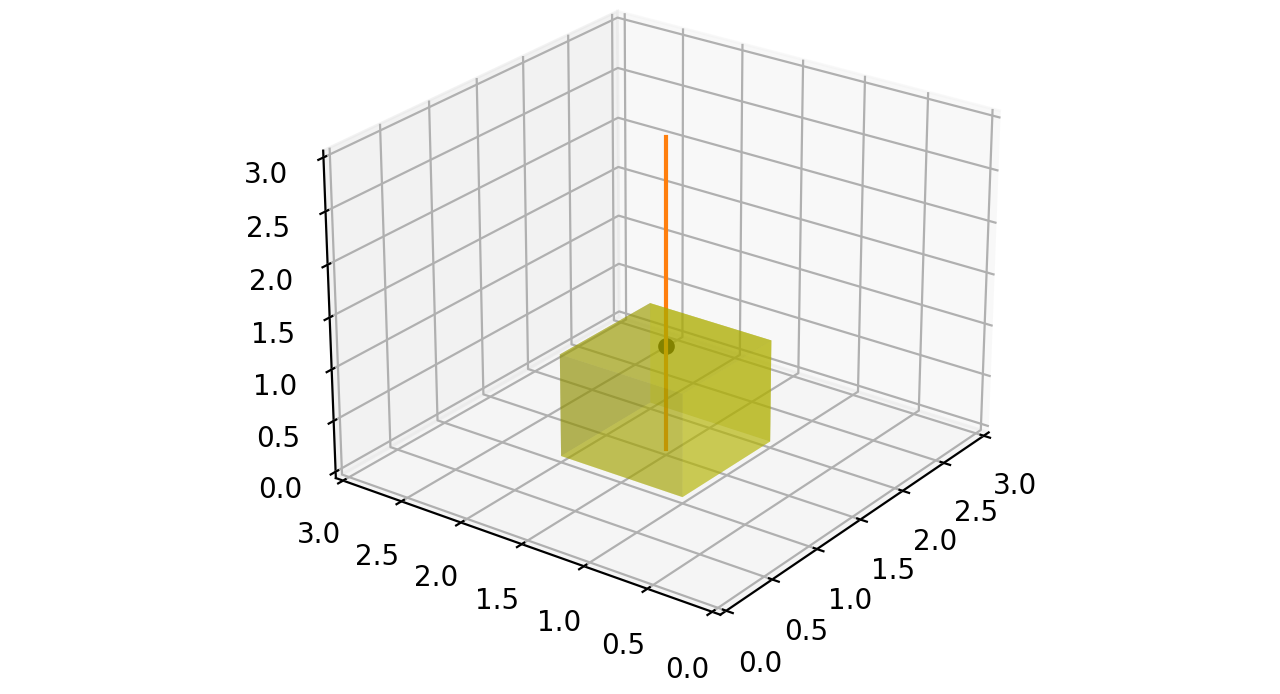
\includegraphics[scale=0.9]{Figure.png}
    \caption{Uniform 2-dimensional PDF and $E[\bm{x}]$}
\end{figure}
Although a bit unclear, the expected value is 
centered inside the uniform probability density function (and the yellow box).
The point along the expected value vector notes where the expected value crosses the c-plane.
Also note that the expected value vector crosses the $X_1X_2$-plane at $(1.5, 1.5)$

\bigskip
\newpage
\textbf{c)} - Find the covariance matrix for $\bm{x}$.
\smallskip

From the definition of the covariance matrix
\begin{equation}
    E[(\bm{x-} \bm{\mu})(\bm{x-} \bm{\mu})^T] = E[\bm{x}\bm{x}^T] - \bm{\mu}\bm{\mu}^T
\end{equation}

The covariance matrix $K_{XX}$ can be calculated such:
\begin{equation}
    K_{{X_i}{X_j}} = E[(X_i - E[X_i])(X_j - E[X_j])]
\end{equation}

Calculating the first diagonal in the covariance matrix:
\begin{equation}
    \begin{aligned}
        E[x_1x_1^T]-\mu_1\mu_1^T = E[x_1^2] - \mu_1^2 =
        \int_{a_1}^{b_1}\frac{x_1^2}{b_1-a_1} dx_1 - \left(\frac{b_1+a_1}{2}\right), \\
        = \left(\frac{a_1^2+a_1b_1+b_1^2}{3}\right)-\left(\frac{a_1+b_1}{2}\right)^2
        =\frac{a_1^2-2a_1b_1+b_1^2}{12} = \frac{(b_1-a_1)^2}{12}
    \end{aligned}
\end{equation}

The same can be done for the second diagonal.

All non-diagonal values in the covariance matrix will be zero. This is due to the fact 
that the continuous uniform PDFs of $X_1$ and $X_2$ are independent of each other, 
and does not affect each other. When the two uniform probability density functions are multiplied 
together to form the multivariable uniform distribution, $X_1$ and $X_2$ is by definition independent.

Thus, the covariance matrix is given as:
\begin{equation}
    K_{XX} = 
    \begin{bmatrix}
        \frac{(b_1-a_1)^2}{12} & 0
        \\ 
        0 & \frac{(b_2-a_2)^2}{12}
    \end{bmatrix}
\end{equation}


\bigskip
\textbf{d)} - Explain the significance of a covariance matrix having identical elements
on the diagonal.
\smallskip

Identical elements on the diagonal means that the random variables $X_1$ and $X_2$ have the same variance.


\bigskip
\textbf{e)} - Explain the significance of a covariance matrix being diagonal.
\smallskip

A covariance matrix being diagonal means that all elements off the diagonal are zero.
This also means that $Cov(X_i, X_j) = 0$ for all $i \neq j$, 
which implies that the vectors are uncorrelated.

\newpage

\problem

A probability density function , $p(\bm{x}), \bm{x} = (x_1, x_2)^T$, has a gaussian distribution around the expected value $\bm{\mu} = (1, 1)^T$ with the covariance matrix
\begin{equation}
    \Sigma = 
    \begin{pmatrix}
        5&3 \\ 
        3&5 
    \end{pmatrix}
\end{equation}

\textbf{a)} - Find the principal axes of the PDF and arrange the eigen vectors 
according to the eigen values in descending order.
\smallskip

\begin{equation}
    \begin{aligned}
        \begin{vmatrix}
            \Sigma - \lambda \textbf{\textit{I}}
        \end{vmatrix}
        =
        \begin{vmatrix}
            \begin{bmatrix}
                5 &3 
                \\ 
                3 & 5
            \end{bmatrix} -
            \lambda
            \begin{bmatrix}
                1 & 0  
                \\ 
                0 & 1
            \end{bmatrix}
        \end{vmatrix}
        =
        \begin{vmatrix}
            5-\lambda&3 \\ 
            3& 5-\lambda
        \end{vmatrix}, \\
        = (5-\lambda)^2-(3)^2
        = \lambda^2-10\lambda+16
        = (\lambda-8)(\lambda-2) = 0
    \end{aligned}
\end{equation}

This gives $\lambda_1 = 8$ and $\lambda_2 = 2$
\begin{equation}
    \Lambda = 
    \begin{pmatrix}
        8&0 \\ 
        0&2
    \end{pmatrix}
\end{equation}

Solving for $\lambda = 8$:
\begin{equation}
    \begin{vmatrix}
        \Sigma - 8\textbf{\textit{I}}
    \end{vmatrix}
    = 
    \begin{vmatrix}
        -3 & 3 \\
        3 & -3
    \end{vmatrix}\bm{x}
    = 0
\end{equation}

\begin{equation}
    \begin{matrix}
        -3x_1 + 3x_2& =& 0 \\ 
        3x_1 + -3x_2&=& 0 \\
        & \Downarrow & \\
        x_1 - x_2 &=& 0
    \end{matrix}
\end{equation}

Which gives the unit vector:
\begin{equation}
    \begin{pmatrix}
        \frac{1}{|\sqrt{1^2+1^2}|} &  \frac{1}{|\sqrt{1^2+1^2}|}
    \end{pmatrix}^T
    =
    \begin{pmatrix}
        \frac{1}{\sqrt{2}} & \frac{1}{\sqrt{2}}
    \end{pmatrix}^T
\end{equation}

Solving for $\lambda = 2$:
\begin{equation}
    \begin{vmatrix}
        \Sigma - 2\textbf{\textit{I}}
    \end{vmatrix}
    = 
    \begin{vmatrix}
        3 & 3 \\
        3 & 3
    \end{vmatrix}\bm{x}
    = 0
\end{equation}

\begin{equation}
    \begin{matrix}
        3x_1 + 3x_2& =& 0 \\ 
        3x_1 + 3x_2&=& 0 \\
        & \Downarrow & \\
        x_1 + x_2 &=& 0
    \end{matrix}
\end{equation}

Which gives the unit vector:
\begin{equation}
    \begin{pmatrix}
        \frac{-1}{|\sqrt{-1^2+1^2}|} &  \frac{1}{|\sqrt{-1^2+1^2}|}
    \end{pmatrix}^T
    =
    \begin{pmatrix}
        -\frac{1}{\sqrt{2}} & \frac{1}{\sqrt{2}}
    \end{pmatrix}^T
\end{equation}

Eigen vector matrix then becomes:
\begin{equation}
    \Phi =
    \begin{pmatrix}
        \frac{1}{\sqrt{2}} & -\frac{1}{\sqrt{2}} \\
        \frac{1}{\sqrt{2}} & \frac{1}{\sqrt{2}}
    \end{pmatrix}
\end{equation}

For verification, it can be shown that:
\begin{equation}
    \bm{\Sigma}
    =
    \begin{pmatrix}
        5&3 \\ 
        3&5
    \end{pmatrix}
    =
    \begin{pmatrix}
        \frac{1}{\sqrt{2}} & -\frac{1}{\sqrt{2}} \\
        \frac{1}{\sqrt{2}} & \frac{1}{\sqrt{2}}
    \end{pmatrix}
    \begin{pmatrix}
        8&0 \\ 
        0&2
    \end{pmatrix}
    \begin{pmatrix}
        \frac{1}{\sqrt{2}} & \frac{1}{\sqrt{2}} \\
        -\frac{1}{\sqrt{2}} & \frac{1}{\sqrt{2}}
    \end{pmatrix}
    =
    \Phi\Lambda\Phi^T
\end{equation}

The first principal axis is therefore:
\begin{equation}
    \sqrt{8}\left(\frac{1}{\sqrt{2}}, \frac{1}{\sqrt{2}}\right)^T = (2, 2)^T
\end{equation}

The second principal axis is then:
\begin{equation}
    \sqrt{2}\left(-\frac{1}{\sqrt{2}}, \frac{1}{\sqrt{2}}\right)^T = (-1, 1)^T
\end{equation}

\bigskip
\textbf{b)} - Sketch the contour lines of $p(\bm{x})$ in the feature space spanned by $\bm{x}$.
Indicate the principal axes and the expected value.
\smallskip

\begin{figure}[H]
    \centering
    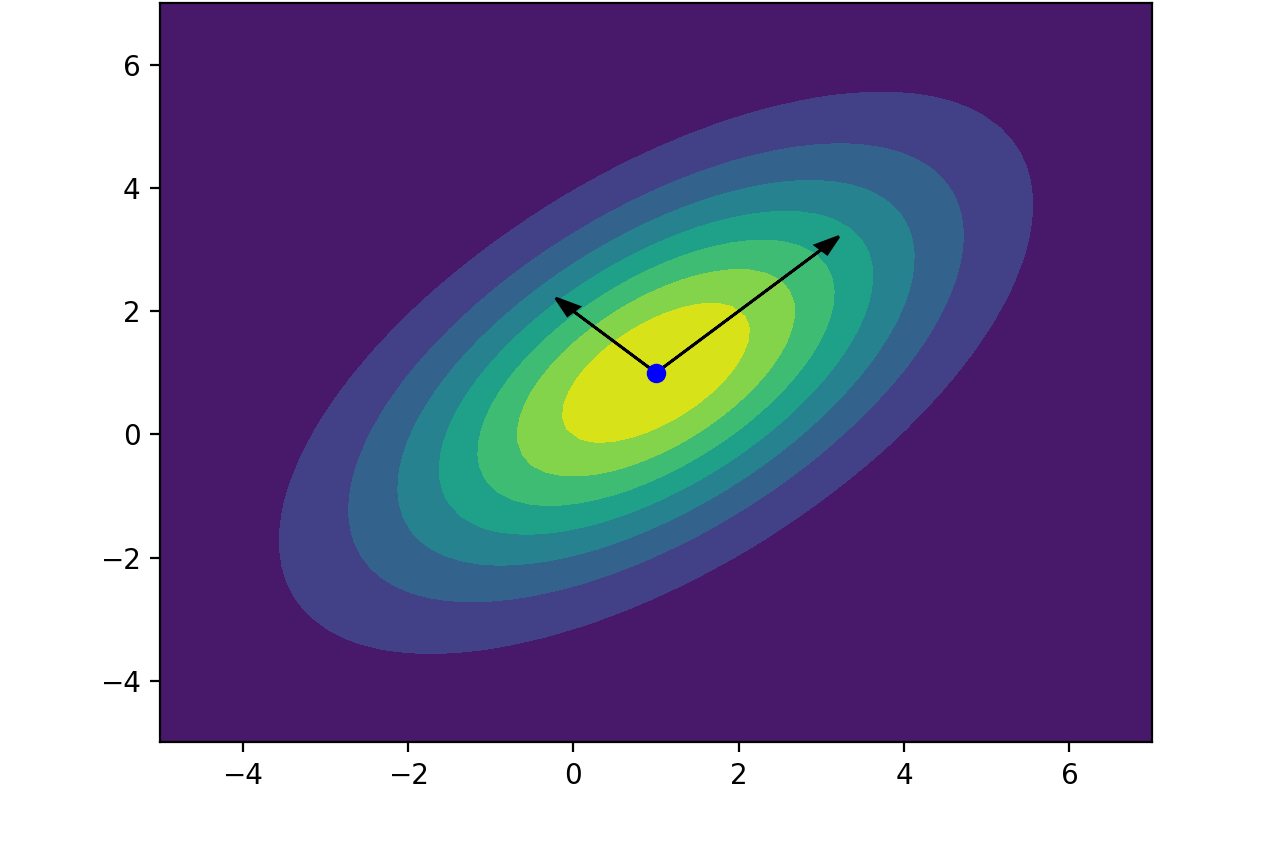
\includegraphics[scale=0.9]{Figure2.png}
    \caption{Contour plot of the gaussian distribution, including $\mu$ and the principal axes}
\end{figure}

\end{document}
